\chapter[Next-generation sequencing describes clonal evolution in interdigitating dendritic cell sarcoma]{Next-generation sequencing describes clonal evolution in interdigitating dendritic cell sarcoma\footnote{This chapter previously published as: Chen HZ\cofirst, Bonneville R\cofirst, \textit{et al}. Genomic characterization of metastatic ultra-hypermutated interdigitating dendritic cell sarcoma through rapid research autopsy. \textit{Oncotarget} 2019, 10(3):277--88.}}
\label{ch:303}

\section{Introduction}
Interdigitating dendritic cell sarcoma (IDCS) is an extremely rare malignancy of dendritic cell origin with approximately 100 cases reported to date \cite{pokuri2015,xue2018}. Due to its rarity and challenging diagnosis, genomic characterization of this neoplasm has not been previously reported. Furthermore, no standard therapy exists for IDCS, which tends to affect middle-age adults with median age of diagnosis of 56.5 years \cite{saygin2013}. Localized IDCS constitutes 47\% of cases and manifests as painless lymphadenopathy, most commonly involving the cervical and axillary nodes. Isolated extra-nodal disease occurs in 25\% of cases, involving the liver, lung, spleen, bone marrow and gastrointestinal tract. Distant metastases occur in 39\% of cases and most frequently involved lymph nodes, lung, liver and bone marrow.

Here we performed whole exome sequencing (WES) of multiple tumors obtained through rapid research autopsy of a patient with metastatic IDCS. To our knowledge, this is the first time IDCS has been extensively sequenced and analyzed. Our findings demonstrate a rare ultra-hypermutated genotype, with \textgreater{}~100 somatic mutations per megabase of genome (muts/Mb) \cite{campbell2017}, characterized by distinct mutational signature profiles and clonal diversity that occurred early in the evolution of this patient's cancer. Phylogenetic analysis revealed inactivation of \textit{TP53} and \textit{CDKN2A} (\textit{p16\textsuperscript{INK4a}/p19\textsuperscript{ARF}}) as well as amplification of \textit{c-KIT} and \textit{PDGFR}$\mathit{\alpha}$ as truncal alterations. We further detected amplification of \textit{APOBEC3A--H} encoding cytidine deaminases on chromosome 22q that may have contributed to the ultra-hypermutation. In summary, our work describes the genomic landscape and clonal heterogeneity of an ultra-rare cancer through the innovative approach of research autopsy. 

\section{Materials and Methods}
\subsection{Research autopsy}
The patient was consented to an Institutional Review Board (IRB)-approved clinical study for tumor profiling and body donation (Figure~\ref{fig:240:autopsy_flowchart}). At time of death, the patient's next-of-kin (and/or hospice agency) notified members of the research team. The deceased was transported to the OSU Medical Center and a limited research autopsy was conducted within 3 hours after patient's passing. Metastatic tumors and adjacent normal tissues were sampled and immediately archived as fresh frozen specimens in OCT medium. After conclusion of the autopsy, the deceased was transported back to the designated funeral home within 24 hours. 

\subsection{Whole exome sequencing}
We extracted genomic DNA from frozen tumors and normal (blood) samples and prepared sequencing libraries using an established protocol \cite{samorodnitsky2015_hyb_amplicon} that included enrichment with the xGen Exome Research Panel v1.0 from Integrated DNA Technologies. Sequencing was performed on an Illumina HiSeq 4000 at The Genomics Services Laboratory at Nationwide Children's Hospital (Columbus, Ohio) and achieved a median depth of 100--286\texttimes{}. 

\subsection{Alignment, variant calling, and annotation}
\label{ssec:303:align_vars_anno}
Sequencing reads were aligned to hg19 using BWA \cite{bwa} version 0.7.14, deduplication using Picard \cite{Picard2019toolkit} version 2.3.0, and quality recalibration and local realignment around indels performed with Picard and GATK \cite{mckenna10} version 3.5 as previously described (Section~\ref{ssec:240:alignment_variant_calling}). Somatic SNVs (single nucleotide variations), somatic indels, and germline SNVs were called using VarScan2 \cite{varscan2} version 2.3.9, filtered using bam-readcount \cite{bamreadcount}, and annotated with ANNOVAR \cite{annovar} (revision \#11f4bb, 2016-02-01) (Section~\ref{ssec:240:alignment_variant_calling}). Mutational signatures from the COSMIC Mutational Signatures set \cite{cosmic_ms} were called with deconstructSigs \cite{rosenthal16} version 1.8.0 with default settings and exome2genome trinucleotide frequency correction, run on R version 3.3.2. Microsatellite instability testing was performed using MANTIS \cite{kautto17} version 1.0.3, run with three threads and otherwise default settings (Section~\ref{ssec:msilandscape:tool_params}). Neighbor-joining trees were computed over the sets of somatic SNVs from all tumor samples as previously described (Section~\ref{ssec:240:nj_methods}). Allele-specific copy number variants (CNVs) were called using FALCON \cite{falcon} followed by manual curation (Section~\ref{ssec:240:cnv_methods}).

\subsection{Subclonal phylogenetic analysis}
\label{ssec:303:phylo_analysis}
The reference read count, alternate allele count, and variant fractions of all nonsynonymous somatic variants called within each tumor sample were compiled as previously described (Section~\ref{ssec:240:canopy_mut_filtering}). As this yielded 893 mutations in this patient, we downsampled to a set of 60 mutations with maximal diversity using a high correlation filter, implemented as follows:
\begin{algorithm}[H]
    \caption{Mutation set downsampling}
    \label{alg:303:mutation_downsampling}
    \begin{algorithmic}[1]
        \While{$|M| > n$}
            \State $i \gets \argmax_x (\rho_{M_x M_y}) \qquad y > x; \quad x,y \in 1 \twodots |M|$
            \State $M \gets M \setminus \{M_i\}$
        \EndWhile
    \end{algorithmic}
\end{algorithm}
\noindent where $M$ is the set of mutations, with each mutation being a vector of its per-sample VFs, $n$ is the desired final number of mutations (in this case, $n = 60$), and $\rho$ is the correlation between VFs in each sample, defined as follows:
\begin{equation}
    \rho_{\vec{a} \vec{b}} = \frac{\cov(\vec{a} \vec{b})}{\sigma_{\vec{a}} \sigma_{\vec{b}}}
\end{equation}
where $\cov(\vec{x}, \vec{y})$ is the covariance between elements of same-length vectors $\vec{x}$ and $\vec{y}$, and $\sigma_{\vec{x}}$ is the population standard deviation of elements of vector $\vec{x}$. Canopy was then run as previously described (Section~\ref{ssec:240:canopy_tree}) followed by \textit{post hoc} assignment of SNVs not used for tree-building (including SNVs removed by downsampling) and indels (Section~\ref{ssec:240:tree_assignment}).

\section{Results}
\subsection{Clinical course}
\begin{figure}[htp]
    \begin{center}
        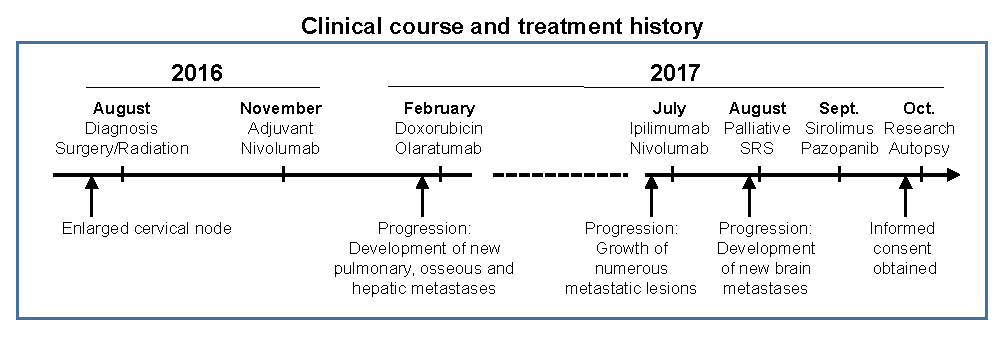
\includegraphics[width=\textwidth,keepaspectratio]{images/303/clinical_course}
    \end{center}
    \vspace{-0.3cm}
    \caption[Clinical course of a patient with metastatic IDCS.]{Clinical course of a patient with metastatic IDCS. Summary of treatment history and tumor response/progression of the patient. Research autopsy was performed 3 hours post-mortem. SRS: stereotactic radiosurgery.}
    \label{fig:303:clinical_course}
\end{figure}
Our patient was a 57-year old Caucasian male who developed an isolated FDG-avid 2.4~\texttimes{}~2.4~cm right-sided neck mass on PET scan in 2016. Biopsy result of this mass showed a ``pleomorphic\slash{}spindle cell neoplasm.'' Immunohistochemical (IHC) analyses demonstrated focal CK7 staining. Clinical evaluation revealed no primary lesion involving the skin or oropharynx. In August 2016, he underwent modified radical right neck dissection and partial submandibular gland excision with one level I lymph node demonstrating complete tumor involvement and suspicious for extranodal extension; remaining lymph nodes (0/29) from levels II, III and IV were negative for tumor infiltration. IHC on the surgical specimen showed positivity for S100, SOX10 and CK7. A diagnosis of IDCS was issued. Given his localized presentation, he received adjuvant radiation to the right level IB--III nodes with a boost to the primary site of disease. In November 2016, he initiated adjuvant nivolumab (3~mg/kg every 2~weeks) given FoundationOne\textsuperscript\textregistered{} report showing \textgreater{}~100~muts/Mb in his tumor. Following adjuvant immunotherapy, he developed metastatic recurrence that failed to respond to subsequent treatments including combination immunotherapy (CTLA-4/PD-1 inhibitors), chemotherapy and molecularly targeted therapies.  His clinical course leading up to the research autopsy is summarized in Figure~\ref{fig:303:clinical_course}.

\begin{figure}[htbp]
	\centering
	\begin{subfigure}{0.72\textwidth}
		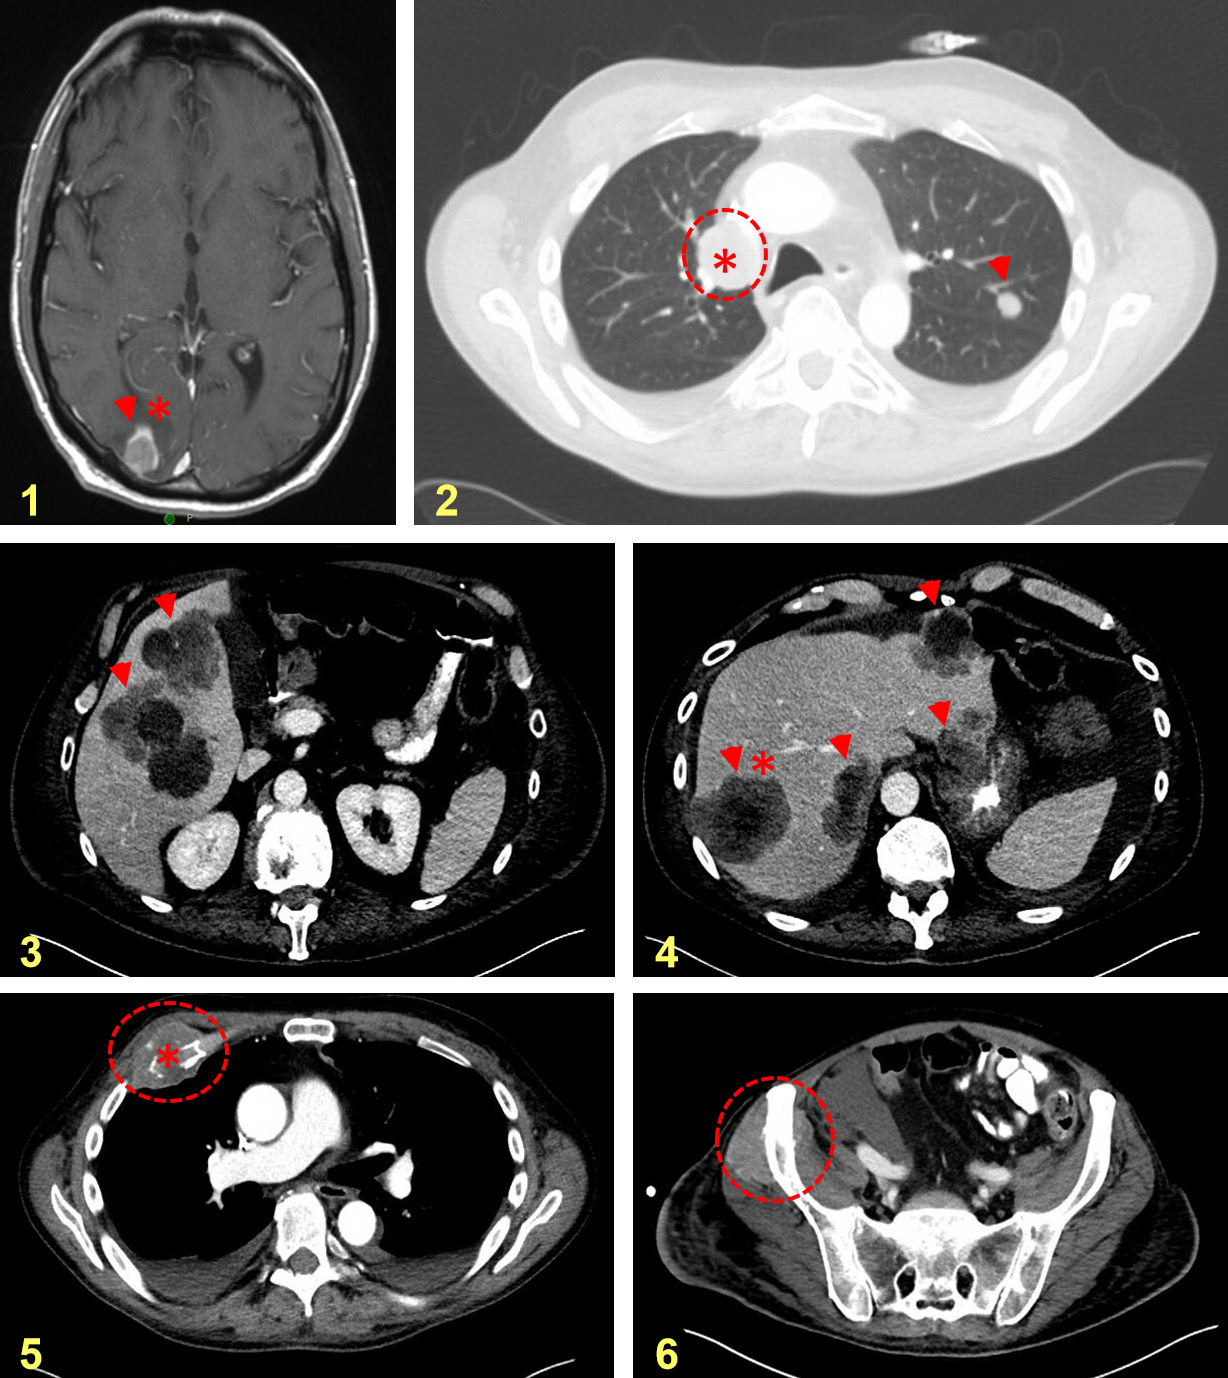
\includegraphics[width=\textwidth,keepaspectratio]{images/303/ct}
		\caption{}\label{fig:303:ct}
	\end{subfigure}%
	\hfill%
	\begin{subfigure}{0.235\textwidth}
		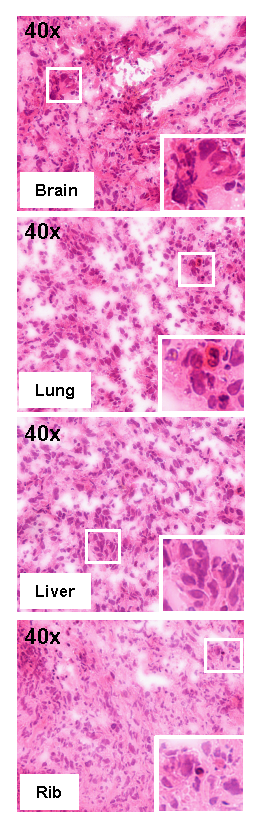
\includegraphics[width=\textwidth,keepaspectratio]{images/303/histo}
		\caption{}\label{fig:303:histo}
	\end{subfigure}
	\caption[Research autopsy of a patient with metastatic IDCS.]{Research autopsy of a patient with metastatic IDCS. (\subref{fig:303:ct}) CT scans depicting organs with metastatic cancer; brain (panel 1, yellow), hilar lymph node (2), liver (3--4), rib (5) and pelvis (6). Arrowheads and dashed circles indicate tumors; asterisks indicate tumors procured at research autopsy. (\subref{fig:303:histo}) H\&E stained frozen sections of metastatic tumors in brain, lung, liver and rib procured from research autopsy. Sections demonstrate high tumor cell content. Enlarged inset at bottom right of each image panel shows dysplastic nuclei with mitotic figures.}
	\label{fig:303:tumor_images}
\end{figure}
Prior to his death, the patient was consented to an IRB-approved research autopsy study for patients with advanced cancers. CT scans obtained prior to hospice enrollment showed tumor involvement of multiple organs (Figure~\ref{fig:303:ct}) and were used to guide sample procurement at time of research autopsy, which was performed within three hours post-mortem. A total of twenty-four metastatic tumor samples were procured from involved organ sites. A pathologist assessed the viability and tumor cell content of autopsy samples (Figure~\ref{fig:303:histo}) prior to selection for genomic studies.

\subsection{Genomic characterization of IDCS}
\begin{table}[ht]
    \centering
    {\footnotesize
    \setlength{\tabcolsep}{2.9pt}
    \begin{tabular}{ccccccccc}
        & \textbf{Organ} & \textbf{\% Tumor} & \textbf{Median} & & \textbf{TMB} & \textbf{\#} & \textbf{\#} & \\
        \textbf{Sample} & \textbf{Involved} & \textbf{Cells} & \textbf{Coverage} & \textbf{\% 100\texttimes{}} & \textbf{(muts/Mb)} & \textbf{SNVs} & \textbf{Indels} & \textbf{MANTIS} \\
        \hline
        T1  & Biopsy (Bx) & 30\%  & 100   & 50.10  & 131.5 & 5,091 & 21    & 0.326 \\
        T2  & Left lung (L.lung) & 80\%  & 213   & 79.83 & 158.4 & 6,139 & 22    & 0.330 \\
        T3  & Right lung (R.lung) & 90\%  & 245   & 84.19 & 165.3 & 6,408 & 19    & 0.330 \\
        T4  & Liver1 & 90\%  & 218   & 82.12 & 163.3 & 6,329 & 20    & 0.328 \\
        T5  & Liver2 & 80\%  & 233   & 83.38 & 158.8 & 6,160 & 15    & 0.327 \\
        T6  & Liver3a & 80\%  & 270   & 87.01 & 150.4 & 5,826 & 22    & 0.318 \\
        T7  & Liver3b & 90\%  & 286   & 87.88 & 156.1 & 6,050 & 19    & 0.324 \\
        T8  & Rib   & 80\%  & 272   & 86.70  & 148.9 & 5,776 & 15    & 0.319 \\
        T9  & Right iliac (R.iliac) & 90\%  & 242   & 85.20  & 167.0   & 6,473 & 20    & 0.330 \\
        T10 & Brain & 50\%  & 257   & 86.80  & 130.1 & 5,043 & 15    & 0.320 \\
    \end{tabular}}
    \caption[Sample characteristics and sequencing metrics.]{Sample characteristics and sequencing metrics. A board-certified pathologist estimated the percentage of tumor cells in each sample. Liver3a and Liver3b samples were procured from two different regions of a large liver tumor. The pre-treatment biopsy sample was obtained from a formalin-fixed paraffin-embedded surgical specimen, while autopsy tumor samples were frozen in OCT\@. \% 100\texttimes{} indicates the percent of variants in each tumor sample with at least 100\texttimes{} coverage. TMB includes synonymous and nonsynonymous SNVs as well as insertions/deletions (indels). \#~SNVs and \#~Indels columns indicate the total number of somatic SNVs and indels detected in each tumor sample. Microsatellite status was determined using MANTIS, with scores \textless{}~0.4 indicating microsatellite stability (MSS).}
    \label{table:303:wes_samples}
\end{table}
We performed WES on nine metastatic tumors and the resected pre-treatment tumor (Table~\ref{table:303:wes_samples}). Calculation of tumor mutational burden (TMB), including single nucleotide variants (SNVs) and insertions/deletions (indels), demonstrated ultra-hypermutation (130.1--167.0~muts/Mb) in all tumors analyzed (Supplemental File~S\thechapter{}.1). Interrogation of microsatellite status utilizing MANTIS \cite{kautto17} showed that all tumors were microsatellite stable (MSS) despite their ultra-hypermutation. 

To further characterize this patient's cancer, we investigated whether specific substitution mutational signatures, which arise due to different mutagenic processes \cite{alexandrov2013}, may be present. This analysis revealed the presence of signature 2 (APOBEC), signature 7 (UV light) and signature 11 (alkylating agent), which are all characterized by C\textgreater{}T substitutions, in all tumor samples (Figure~\ref{fig:303:mutational_spectra_by_sample}, Supplemental File~S\thechapter{}.2). Of the three mutational signatures, signature 7 had the highest prevalence.

\begin{figure}[htbp]
	\centering
	\begin{subfigure}{0.23\textwidth}
		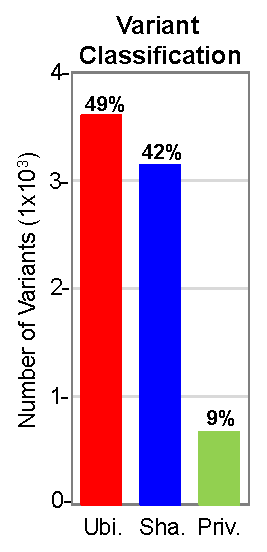
\includegraphics[width=\textwidth,keepaspectratio]{images/303/variants_by_category}
		\caption{}\label{fig:303:variants_by_category}
	\end{subfigure}%
	\hfill%
	\begin{subfigure}{0.72\textwidth}
		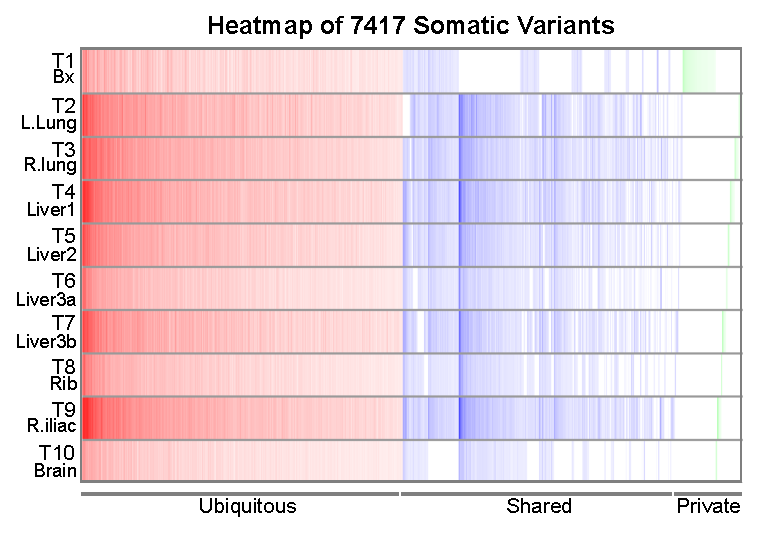
\includegraphics[width=\textwidth,keepaspectratio]{images/303/mutation_heatmap}
		\caption{}\label{fig:303:mutation_heatmap}
	\end{subfigure}\par\vspace{0.3cm}
	\begin{subfigure}{0.9\textwidth}
	    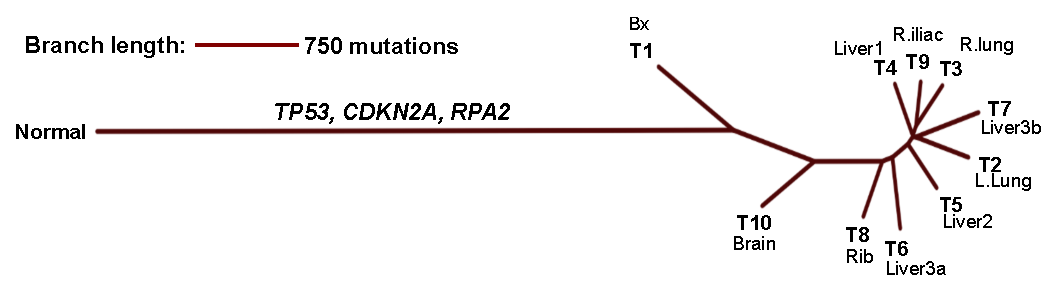
\includegraphics[width=\textwidth,keepaspectratio]{images/303/nj_tree}
	    \caption{}\label{fig:303:nj_tree}
	\end{subfigure}
	\caption[Classification of somatic variants and NJ tree.]{Classification of somatic variants and construction of neighbor joining (NJ) tree. (\subref{fig:303:variants_by_category}) The 7,417 somatic variants detected in all ten tumor samples T1--10 from this patient were classified into three categories: Ubiquitous (Ubi.), present in all ten tumor samples; Shared (Sha.), present in some but not all ten tumor samples; Private (Priv.), present in only one tumor sample. Percentage of each variant category are as indicated in the bar graph. Somatic variants analyzed include single nucleotide variants (SNVs) and insertions/deletions (indels). (\subref{fig:303:mutation_heatmap}) Heatmap demonstrating distribution and variant allele frequency (VAF) of the 7,417 somatic variants in ten tumor samples T1--10. Color intensity corresponds to VAF\@. (\subref{fig:303:nj_tree}) NJ tree depicting the evolutionary relationship of the ten tumor samples T1--10 from this patient. Normal represents hypothetical population of wild-type cells without somatic aberrations. The 3,642 ubiquitous variants included driver mutations in \textit{TP53} and \textit{CDKN2A} as well as the \textit{RPA2} variant predicted to have loss-of-function. Branch lengths correspond to the genetic distance between samples. T1--10 correspond to samples listed in Table~\ref{table:303:wes_samples}.}
	\label{fig:303:variants_plots}
\end{figure}
We next classified the 7,417 somatic variants (SNVs and indels) in all ten tumor samples of this patient into three categories: Ubiquitous, Shared, and Private (Figure~\ref{fig:303:variants_plots}). Ubiquitous variants are variants detected in all tumor samples and included driver mutations in \textit{TP53} and \textit{CDKN2A}, while shared variants are those detected in subsets of tumor samples. Finally, private variants are variants unique to each tumor sample. A tumor-centric evolutionary tree was constructed based on the pairwise genetic distance, as measured by number of discordant SNVs, between the wild-type cells (normal) and tumor samples in this patient (Figure~\ref{fig:303:nj_tree}). Finally, we interrogated the prevalence of copy number variations (CNVs) using the allele-specific CNV caller FALCON. After manual review and curation, 29 unique CNVs including amplification (including \textit{c-KIT}, \textit{PDGFR}$\mathit{\alpha}$, and \textit{APOBEC3A--H}), deletion and loss-of-heterozygosity events were detected (Figure~\ref{fig:303:cnv_plots} and Supplemental Files~S\thechapter{}.3--4).

\subsection{Reconstructing clonal evolution}
\label{ssec:303:clone_results}
\begin{figure}[htbp]
	\centering
	\begin{subfigure}{0.4\textwidth}
		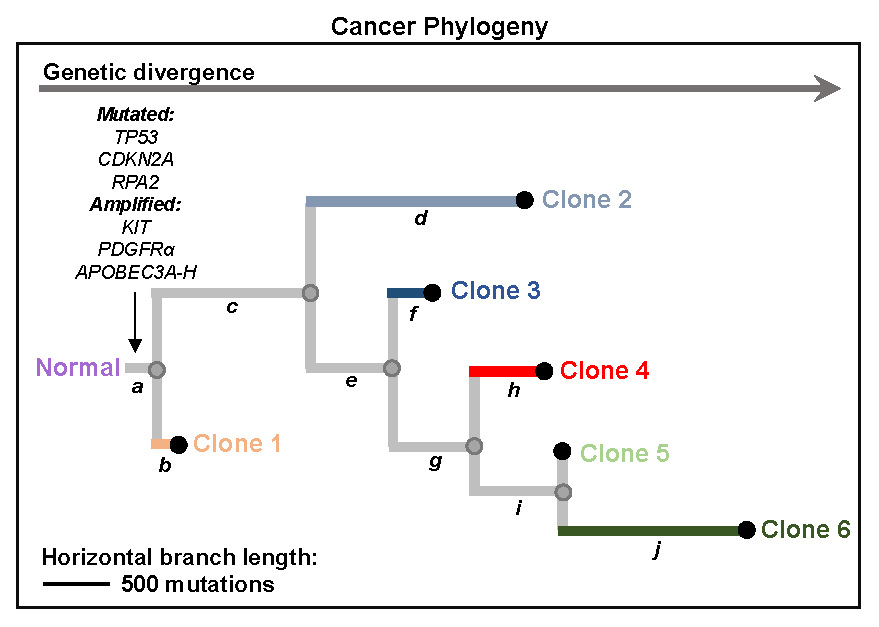
\includegraphics[width=\textwidth,keepaspectratio]{images/303/canopy_tree}
		\caption{}\label{fig:303:canopy_tree}
	\end{subfigure}%
	\hfill%
	\begin{subfigure}{0.55\textwidth}
	    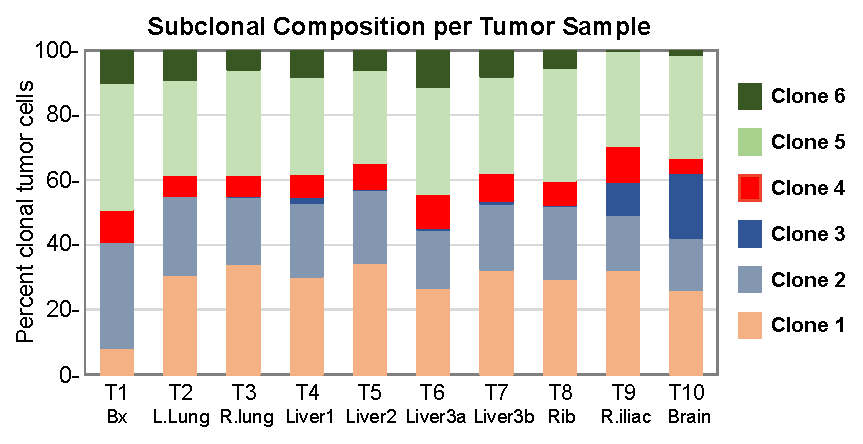
\includegraphics[width=\textwidth,keepaspectratio]{images/303/canopy_P}
	    \caption{}\label{fig:303:canopy_P}
	\end{subfigure}\par\vspace{0.1cm}
	\begin{subfigure}{0.5\textwidth}
	    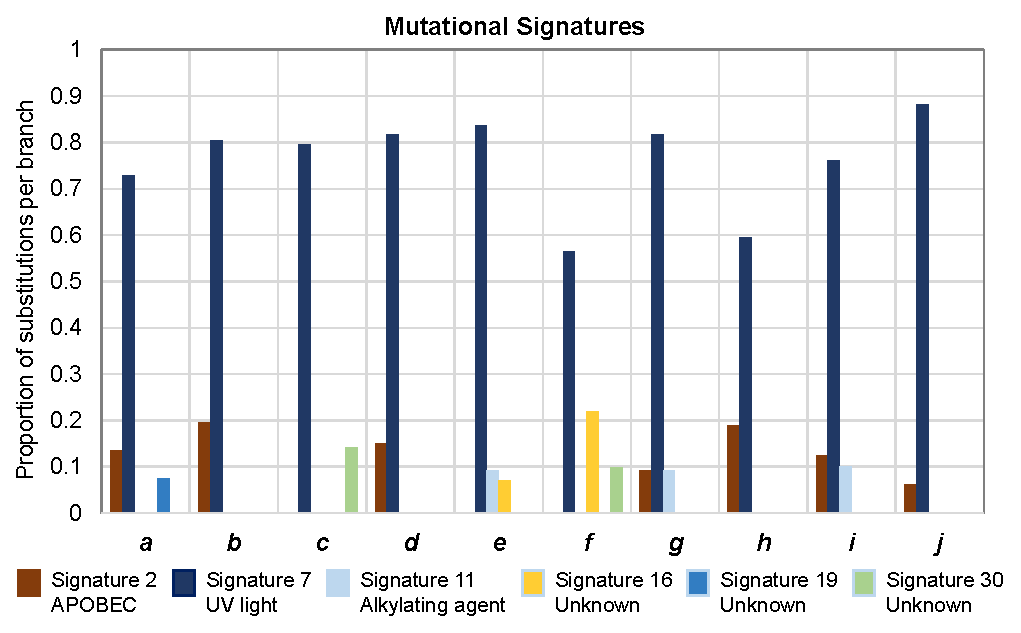
\includegraphics[width=\textwidth,keepaspectratio]{images/303/sigs_per_branch}
	    \caption{}\label{fig:303:sigs_per_branch}
	\end{subfigure}
	\caption[Analysis of cancer phylogeny and clonal evolution.]{Analysis of cancer phylogeny and clonal evolution. (\subref{fig:303:canopy_tree}) Phylogram constructed using Canopy integrating SNVs, curated CNVs and indels detected through WES of tumor samples T1--10. Output from Canopy includes number of clones, clonal fractions and mutational groups (\textbf{\textit{a--j}}) associated with each clone. Given the large number of somatic SNVs in this ultra-hypermutated cancer, downsampling of SNVs was performed in addition to following recommended parameters for Canopy tree building. Somatic SNVs not utilized by Canopy as well as indels were retroactively assigned based on VAF patterns to mutational groups \textbf{\textit{a--j}} using a maximal likelihood model. Based on this analysis, six different clones of tumor cells were identified in this patient's cancer. Truncal or group a mutations are common or ancestral to all clones of tumor cells. In contrast, mutations in groups \textbf{\textit{b}}, \textbf{\textit{d}}, \textbf{\textit{f}}, \textbf{\textit{h}}, and \textbf{\textit{j}} are private to clones 1, 2, 3, 4, and 6, respectively. The length of horizontal branches in the tree is proportional to the number of mutations. (\subref{fig:303:canopy_P}) Stacked bar graph depicting the percentage of different clonal tumor cell populations as estimated by Canopy in each sample. (\subref{fig:303:sigs_per_branch}) Mutations in each branch of the phylogram estimated by Canopy were called with deconstructSigs, utilizing the COSMIC Mutational Signatures set. Signature 7 (UV) was detected in every branch of the tumor's evolutionary history. T1--10 correspond to samples listed in Table~\ref{table:303:wes_samples}.}
	\label{fig:303:canopy_results}
\end{figure}
Integrating the above genomic data (SNVs, indels and CNVs), we used the program Canopy \cite{canopy} to synthesize a hypothetical model of the clonal evolution of this patient's cancer (Figure~\ref{fig:303:canopy_tree}). Canopy identified six genetically distinct clonal populations of tumor cells, present in various proportions within each tumor (Figure~\ref{fig:303:canopy_P}, Supplemental File~5). These six clones are differentiated by ten unique groups of genomic alterations (\textbf{\textit{a--j}}, Supplemental Files~S\thechapter{}.6--7), which all contained mutational signature 7 (Figure~\ref{fig:303:sigs_per_branch} and Supplemental File~S\thechapter{}.2). Of note, group \textbf{\textit{a}} contains truncal alterations ancestral to all tumor cells including two well-documented driver mutations, \textit{TP53} P278L and \textit{CDKN2A} R80X, which were classified as ubiquitous. Interestingly, we also detected a truncal variant \textit{RPA2} V108L\@. \textit{RPA2} encodes a subunit of the heterotrimeric Replication Protein A complex that is critical for DNA replication, repair, recombination and DNA damage response \cite{byrne2019}. Finally, we identified two notable truncal amplifications of regions on the long arms of chromosome 4 (\textapprox{}17.2~Mb), containing \textit{c-KIT} and \textit{PDGFR}$\mathit{\alpha}$, and chromosome 22 (\textapprox{}24.6~Mb), containing \textit{APOBEC3A--H} (Figure~\ref{fig:303:cnv_plots}).

\section{Discussion}
Extensive multi-regional sequencing of tumors revealed the complex genetic landscape of treatment-refractory cancers by demonstrating intratumor heterogeneity \cite{gerlinger2012,gerlinger2014}, which underscores the limitations of tumor profiling with tissue derived from a single biopsy specimen. From a clinical perspective, tumor heterogeneity contributes to the incomplete therapeutic responses seen in patients receiving different types of anti-cancer therapies including molecularly targeted therapies. Mechanistically, tumor heterogeneity drives acquired therapeutic resistance by facilitating the selection and expansion of therapy-resistant clones. Research autopsy has emerged as a powerful approach to characterize tumor heterogeneity at different metastatic sites in the individual patient. Together with information from treatment-na\"ive samples, sequencing of metastatic tumor samples from autopsy can provide a comprehensive molecular portrait of advanced cancers that reflects changes in tumor cell populations and genomes over time \cite{faltas2016,juric2015}. Here we performed research autopsy on a patient with widely metastatic IDCS. Genomic profiling of his tumors revealed somatic ultra-hypermutation and tumor heterogeneity in the form clonal diversity. Recently, Campbell \textit{et al} demonstrated a prevalence of ultra-hypermutation (TMB \textgreater{}~100~muts/Mb) of 0.6\% in a cohort of 78,452 adult cancers \cite{campbell2017}. Therefore, the rare histologic classification of IDCS in this patient is accompanied by a rare `genotype' of ultra-hypermutation.

Hypermutation in cancer may arise from intrinsic defects in DNA damage repair pathways or extrinsic mechanisms such as mutagenic exposure \cite{campbell2017}. The majority of ultra-hypermutation detected by Campbell et al. was attributed to mutations in mismatch repair (MMR) genes and replication-associated DNA polymerases POL$\varepsilon$ or POL$\delta$ (Section~\ref{ssec:intro:dna_replication}--\ref{ssec:intro:mutation}). While we did not detect genomic alterations involving MMR or POL$\varepsilon$\slash{}POL$\delta$ to explain this patient's ultra-hypermutated cancer, we did detect a truncal amplification of a region on chromosome 22q containing genes encoding the APOBEC3A--H (or A3 subfamily) cytidine deaminases. The deregulated expression and activity of A3A and A3B have been linked to cancer development through enhanced DNA hypermutation and unfaithful RNA editing \cite{salter2016,burns2013,henderson2015}. Furthermore, we identified a truncal \textit{RPA2} variant with a predicted (by DUET \cite{pires2014}) destabilizing missense mutation in the C-terminal winged helix domain important for protein-protein interaction that could have further contributed to defective DNA damage repair and hypermutation. Together with driver mutations in tumor suppressors \textit{TP53} and \textit{CDKN2A}, the above events could have produced ultra-hypermutation as seen in this patient's cancer.

Different models of mutation accumulation have been proposed for hypermutated cancers and could be classified as `steady' versus `dynamic' hypermutation \cite{campbell2017}. In the steady model, mutations accumulate gradually due to continuous mutagenic exposure or germline MMR deficiencies, leading to hypermutation over time. The dynamic model, seen in cancers with POL$\varepsilon$ or POL$\delta$ mutations, is characterized by `bursts' of mutations followed by rise in genome-wide TMB. Through analyses of clonality and mutational signatures, we hypothesize a gradual mode of hypermutation consistent with the former model in our patient's cancer. Genomic profiling of treatment-na\"ive tumor revealed high TMB at baseline that may have been the result of UV exposure, producing the driver mutations in \textit{TP53} and \textit{CDKN2A}\@. TMB analysis of his autopsy tumor samples demonstrated an increase of \textapprox{}20--37 additional muts/Mb that could be attributed to the truncal amplification of the A3 subfamily of cytidine deaminases, as indicated by the presence of APOBEC-specific signature 2, and/or potentially therapy-induced mutations. Interestingly, the brain metastasis (T10) was the only autopsy tumor sample that had similar TMB as the treatment-na\"ive tumor (T1) while still retaining the APOBEC signature. A technical explanation underlying this finding may be due to lower tumor cell contents in both samples affecting variant detection. Alternatively, this may reflect similar biology between the treatment-na\"ive tumor sample obtained from neck surgery and the brain metastasis; this similarity is demonstrated by the shorter genetic distance between `normal' and T1 or T10 samples relative to other tumor samples in the NJ tree. Finally, the genetic dissimilarity between the brain metastasis and tumor samples from other organs also suggests the presence of unique genetic features of cancer cells with increased propensity for invasion of the central nervous system. Although high TMB has been established as a clinically useful biomarker of response to checkpoint blockade in multiple human cancers \cite{yarchoan2017,gibney2016}, our patient developed progressive cancer while receiving adjuvant therapy with the PD-1 inhibitor nivolumab and had disease progression while being treated with dual \mbox{CTLA-4/PD-1} blockade. Therefore, his case highlights the need for identification of additional biomarkers to predict clinical benefit for immunotherapy in patients with hypermutated cancers.

In summary, we present the first genomic characterization of metastatic IDCS, an extremely rare neoplasm of dendritic cell origin that lacks any standard therapy. This patient had metastatic IDCS characterized by ultra-hypermutation and clonal heterogeneity, likely through a combination of chronic mutagen exposure (UV), acquired defects in pathways important for DNA repair (\textit{TP53}, \textit{CDKN2A}, \textit{RPA} mutations), and gain of genes that promote DNA hypermutation (\textit{APOBEC3A--H})\@. His cancer was aggressive and refractory to multiple anti-cancer therapies including molecularly targeted agents and immunotherapies. In the future, it will be important to study additional patients with this and other rare cancers with hypermutation. Finally, the broader clinical implication of our results is that although patients with hypermutated cancer, originating from either somatic or germline genomic aberrations, are more likely to benefit from checkpoint inhibition, research is still needed to stratify these patients to maximize therapeutic efficacy and identify the different genetic determinants of primary or acquired resistance to immunotherapy.

\section{List of Supplemental Files}
All supplemental files are available at \url{https://github.com/rbonneville/PhD-Dissertation/}.
\begin{enumerate}
    \renewcommand*{\labelenumi}{S\thechapter{}.\arabic{enumi}. }
    \item Annotated mutations by tumor sample. SNVs and indels passing quality control filters (Section~\ref{ssec:303:align_vars_anno}) were annotated using ANNOVAR.
    \item Mutational signatures per tumor and per phylogeny branch. Mutations in each tumor and each branch were called with deconstructSigs, utilizing the COSMIC Mutational Signatures set.
    \item Allele-specific CNVs were called using FALCON with the QC procedure provided with Canopy. Output prior to manual curation is provided in this file.
    \item For each of the 29 CNV-affected regions identified and manually curated, the major and minor copy number and standard deviations are listed. These values were determined through execution of FALCON with manual selection of SNVs for segmentation.
    \item Estimated clonal composition of all tumor samples. For each of 10 tumor samples, the estimated fraction of normal and tumor cells from each clone is listed.
    \item Annotated mutations by phylogeny branch. SNVs and indels are listed for each branch \textbf{\textit{a--j}} of the phylogram (Figure~\ref{fig:303:canopy_tree}). Mutations in bold were used by Canopy to build the tree, and the remaining mutations were retroactively assigned to the tree (Section~\ref{ssec:303:phylo_analysis}).
    \item Curated CNVs by phylogeny branch. For each of the 29 CNV-affected regions identified and manually curated, the per-subclone major and minor copy number as estimated by Canopy is listed.
\end{enumerate}

\section*{Acknowledgements}
We are grateful for administrative support from Jenny Badillo, the Comprehensive Cancer Center, community support from Pelotonia, and most importantly the patient and his family. We thank the Ohio Supercomputer Center (OSC) for providing us with the computing power and resources for the analyses in this report.
